\documentclass[a4paper,12pt]{article}
\usepackage[top = 2.5cm, bottom = 2.5cm, left = 2.5cm, right = 2.5cm]{geometry}
\usepackage[T1]{fontenc}
\usepackage[utf8]{inputenc}
\usepackage{multirow} 
\usepackage{booktabs} 
\usepackage{graphicx}
\usepackage[spanish]{babel}
\usepackage{setspace}
\setlength{\parindent}{0in}
\usepackage{float}
\usepackage{fancyhdr}
\usepackage{amsmath}
\usepackage{amssymb}
\usepackage{amsthm}
\usepackage[numbers]{natbib}
\newcommand\Mycite[1]{%
	\citeauthor{#1}~[\citeyear{#1}]}
\usepackage{graphicx}
\usepackage{subcaption}
\usepackage{booktabs}
\usepackage{etoolbox}
\usepackage{minibox}
\usepackage{hyperref}
\usepackage{xcolor}
\usepackage{pdfpages}
\usepackage[skins]{tcolorbox}
%---------------------------

\newtcolorbox{cajita}[1][]{
	 #1
}

\newenvironment{sol}
{\renewcommand\qedsymbol{$\square$}\begin{proof}[\textbf{Solución.}]}
	{\end{proof}}

\newenvironment{dem}
{\renewcommand\qedsymbol{$\blacksquare$}\begin{proof}[\textbf{Demostración.}]}
	{\end{proof}}

\newtheorem{problema}{Problema}
\newtheorem{definicion}{Definición}
\newtheorem{ejemplo}{Ejemplo}
\newtheorem{teorema}{Teorema}
\newtheorem{corolario}{Corolario}[teorema]
\newtheorem{lema}[teorema]{Lema}
\newtheorem{prop}{Proposición}
\newtheorem*{nota}{\textbf{NOTA}}
\renewcommand\qedsymbol{$\blacksquare$}
\usepackage{svg}
\usepackage{tikz}
\usepackage[framemethod=default]{mdframed}
\global\mdfdefinestyle{exampledefault}{%
linecolor=lightgray,linewidth=1pt,%
leftmargin=1cm,rightmargin=1cm,
}




\newenvironment{noter}[1]{%
\mdfsetup{%
frametitle={\tikz\node[fill=white,rectangle,inner sep=0pt,outer sep=0pt]{#1};},
frametitleaboveskip=-0.5\ht\strutbox,
frametitlealignment=\raggedright
}%
\begin{mdframed}[style=exampledefault]
}{\end{mdframed}}
\newcommand{\linea}{\noindent\rule{\textwidth}{3pt}}
\newcommand{\linita}{\noindent\rule{\textwidth}{1pt}}

\AtBeginEnvironment{align}{\setcounter{equation}{0}}
\pagestyle{fancy}

\fancyhf{}









%----------------------------------------------------------
\lhead{\footnotesize Data Science I}
\rhead{\footnotesize  Rudik Roberto Rompich}
\cfoot{\footnotesize \thepage}


%--------------------------

\begin{document}
 \thispagestyle{empty} 
    \begin{tabular}{p{15.5cm}}
    \begin{tabbing}
    \textbf{Universidad del Valle de Guatemala} \\
    Departamento de Ciencias de la Computación\\\\
   \textbf{Estudiantes:} Augusto Alonso, Angel Cuellar, Rudik Roberto Rompich\\
    \end{tabbing}
    \begin{center}
        CC3066 - Data Science I - Catedrático: Luis Furlan\\
        \today
    \end{center}\\
    \hline
    \\
    \end{tabular} 
    \vspace*{0.3cm} 
    \begin{center} 
    {\Large \bf  Proyecto 2 - Análisis Exploratorio 
} 
        \vspace{2mm}
    \end{center}
    \vspace{0.4cm}
%--------------------------

\textbf{Instrucciones: } en clase vimos un modelo simple de una red neuronal utilizando \textit{TensorFlow} 2. Utilizando el código desarrollado (o si lo desea uno propio pero que funcione correctamente), responda a las siguientes preguntas:

\begin{problema}
	Cambie el número de observaciones a 100,000. ¿Qué ocurre?
\end{problema}
\begin{sol}
	Los resultados a simple vista parecen ser lo mismos; tales que 
	\begin{enumerate}
		\item La cantidad de observaciones hace que el modelo sea un poco más lento y mucho más tardado.
		\item El error parece estabilizarse bastante más rápido y converge aproximadamente a un mismo número. 
		\item Los pesos y sesgos no variaron en nada, se mantienen cercanos a las cifras esperadas. 
		\item La gráfica del problema sigue la misma tendencia (solo que con más datos). 
		\item Cabe recalcar que estamos en un caso de \textit{overfitting} ya que se usaron los mismos datos de entrenamiento. 
		\item La gráfica: 
		\begin{figure}[H]
			\centering 
			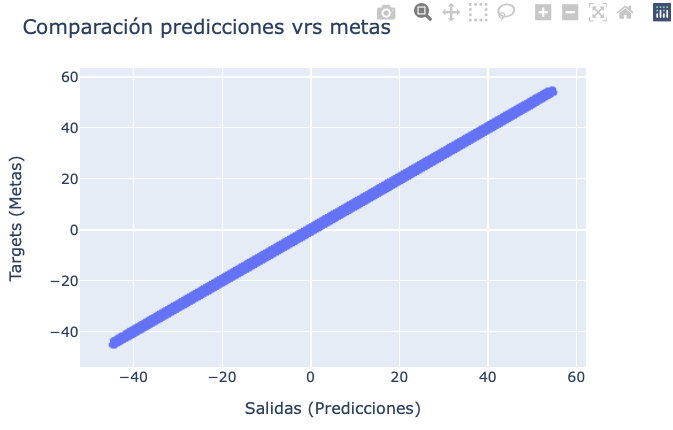
\includegraphics[scale=0.4]{Images/1}
		\end{figure}
	\end{enumerate}
\end{sol}

\begin{problema}
	«Juegue» un poco con la tasa de aprendizaje. Los valores como 0.0001, 0.001, 0.1, 1 son interesantes para observar ¿Qué diferencias se observan? ¿Se comporta bien el algoritmo?
\end{problema}
\begin{sol} Tenemos los siguientes casos: 
	\begin{enumerate}
		\item[\textbf{0.0001}] (1) El algoritmo arroja pesos y sesgos bastante precisos. (2) El algoritmo tomó un poco más de tiempo en ejecutarse, comparado a la tasa de aprendizaje anterior. (3) La pérdida se estabilizó completamente en 0.3323. 
		\item[\textbf{0.001}] (1) El algoritmo arroja pesos y sesgos bastante precisos (aunque por décimas impreciso a lo esperado). (2) El algoritmo fue un poco más eficiente en ejecutarse, comparado a la tasa de aprendizaje del inciso anterior. (3) La pérdida se estabilizó completamente en 0.3333. 
		\item[\textbf{0.1}] El modelo explotó; la tasa de aprendizaje es muy grande.
		\item[\textbf{1}]  El modelo explotó; la tasa de aprendizaje es muy grande.
	\end{enumerate}
\end{sol}
\begin{problema}
	Cambie la función de pérdida. Una función altenativa es la "Huber Loss". \bigbreak 
La función de pérdida Huber es más adecuada que la L2.norm cuando tenemos valores atípicos, ya que es menos sensitiva a los mismos (en nuestro ejemplo no tenemos valores atípicos, pero seguramente se topará con ellos en el futuro). La L2-norm eleva todas las diferencias al cuadrado, por lo que los valores atípicos tienen mucha influencia sobre los resultados. La sintáxis correcta de la función de pérdida Huber es "huber\_loss".
\bigbreak 
	¿Cómo se comparan los resultados al cambiar la función de pérdida?
\end{problema}
\begin{sol}
	Por los datos de entrenamiento «idealistas» que se usaron para hacer las predicciones, ya que fueron los mismos que para la construcción del modelo; se pensaría que no habría un efecto directo en los resultados. Sin embargo, con una tasa de aprendizaje de 0.02 se produce la siguiente gráfica, con los puntos más homogéneamente distribuidos: 
	\begin{figure}[H]
		\centering 
		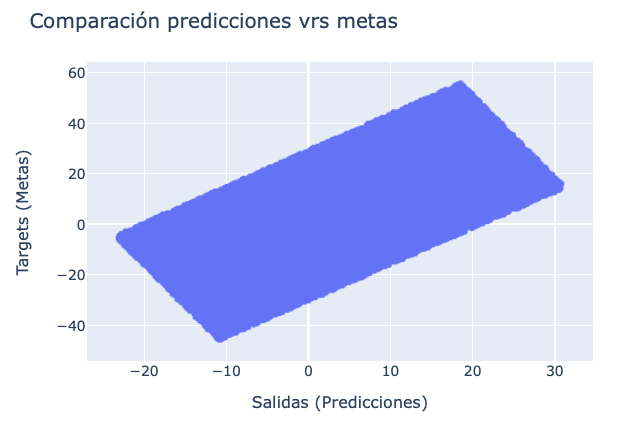
\includegraphics[scale=0.4]{Images/2}
	\end{figure}
	
\end{sol}

Referencia:
https://www.tensorflow.org/versions/r1.15/api\_docs/python/tf/keras

%---------------------------


\end{document}